\subsection{The Chessboard Encoding Problem}

This problem is from a collaboration between 3blue1brown and Matt Parker. I attempted this problem years ago, but could not do it, but on a second attempt recently I got it instanteously. I think I spoiled this problem for myself however as I had watched a video recently about a highly relevant problem, and I would never have got it so fast otherwise. I give this problem a difficulty of 5/10, although the ideas behind the solution did lead to someone winning the Turing Prize.

You and a colleague are inprisoned, although the prison warden gives you an opportunity for freedom. There is an $8 \times 8$ chessboard where each square is a hidden compartment, and the warden reveals to one of you, let us call them person A, which square the key to the door is hidden in. A coin is then placed on each square in a configuration decided by the warden that is not known to you or your colleague in advance. Person A has to turn over exactly one coin before leaving the room, at which point person B enters and needs to determine which square has the key. You are allowed to agree a strategy beforehand, although the warden will hear your strategy, and will try and find a configuration of coins to make your strategy not work.

\textbf{Hints:}

\begin{enumerate}
	\item Consider a board with two squares, then four squares.
	\item There exists a reliable strategy if and only if the number of squares is a power of two~\cite{}.
	\item Consider the parity of the number of coins that are heads-up in a region.
\end{enumerate}

\textbf{Solution:}

The solution works by being able to control the parity of the number of heads-up coins in six regions. This produces a six-digit binary number which can be used to encode the square of the chessboard as $8 \times 8 = 64 = 2^6$. The key is to be able to control the parity in each region indepently, and the six regions shown in figure~\ref{} allow this.

\begin{figure}[H]
	\begin{center}
		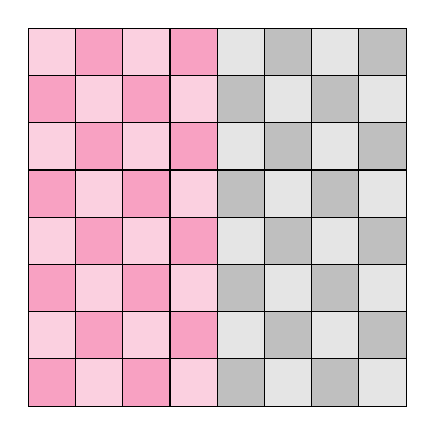
\begin{tikzpicture}[scale=0.6]
			\draw[fill=WildStrawberry, fill opacity=0.4] (0, 0) -- (0, 1) -- (1, 1) -- (1, 0) -- (0, 0);
\draw[fill=WildStrawberry, fill opacity=0.2] (0, 1) -- (0, 2) -- (1, 2) -- (1, 1) -- (0, 1);
\draw[fill=WildStrawberry, fill opacity=0.4] (0, 2) -- (0, 3) -- (1, 3) -- (1, 2) -- (0, 2);
\draw[fill=WildStrawberry, fill opacity=0.2] (0, 3) -- (0, 4) -- (1, 4) -- (1, 3) -- (0, 3);
\draw[fill=WildStrawberry, fill opacity=0.4] (0, 4) -- (0, 5) -- (1, 5) -- (1, 4) -- (0, 4);
\draw[fill=WildStrawberry, fill opacity=0.2] (0, 5) -- (0, 6) -- (1, 6) -- (1, 5) -- (0, 5);
\draw[fill=WildStrawberry, fill opacity=0.4] (0, 6) -- (0, 7) -- (1, 7) -- (1, 6) -- (0, 6);
\draw[fill=WildStrawberry, fill opacity=0.2] (0, 7) -- (0, 8) -- (1, 8) -- (1, 7) -- (0, 7);
\draw[fill=WildStrawberry, fill opacity=0.2] (1, 0) -- (1, 1) -- (2, 1) -- (2, 0) -- (1, 0);
\draw[fill=WildStrawberry, fill opacity=0.4] (1, 1) -- (1, 2) -- (2, 2) -- (2, 1) -- (1, 1);
\draw[fill=WildStrawberry, fill opacity=0.2] (1, 2) -- (1, 3) -- (2, 3) -- (2, 2) -- (1, 2);
\draw[fill=WildStrawberry, fill opacity=0.4] (1, 3) -- (1, 4) -- (2, 4) -- (2, 3) -- (1, 3);
\draw[fill=WildStrawberry, fill opacity=0.2] (1, 4) -- (1, 5) -- (2, 5) -- (2, 4) -- (1, 4);
\draw[fill=WildStrawberry, fill opacity=0.4] (1, 5) -- (1, 6) -- (2, 6) -- (2, 5) -- (1, 5);
\draw[fill=WildStrawberry, fill opacity=0.2] (1, 6) -- (1, 7) -- (2, 7) -- (2, 6) -- (1, 6);
\draw[fill=WildStrawberry, fill opacity=0.4] (1, 7) -- (1, 8) -- (2, 8) -- (2, 7) -- (1, 7);
\draw[fill=WildStrawberry, fill opacity=0.4] (2, 0) -- (2, 1) -- (3, 1) -- (3, 0) -- (2, 0);
\draw[fill=WildStrawberry, fill opacity=0.2] (2, 1) -- (2, 2) -- (3, 2) -- (3, 1) -- (2, 1);
\draw[fill=WildStrawberry, fill opacity=0.4] (2, 2) -- (2, 3) -- (3, 3) -- (3, 2) -- (2, 2);
\draw[fill=WildStrawberry, fill opacity=0.2] (2, 3) -- (2, 4) -- (3, 4) -- (3, 3) -- (2, 3);
\draw[fill=WildStrawberry, fill opacity=0.4] (2, 4) -- (2, 5) -- (3, 5) -- (3, 4) -- (2, 4);
\draw[fill=WildStrawberry, fill opacity=0.2] (2, 5) -- (2, 6) -- (3, 6) -- (3, 5) -- (2, 5);
\draw[fill=WildStrawberry, fill opacity=0.4] (2, 6) -- (2, 7) -- (3, 7) -- (3, 6) -- (2, 6);
\draw[fill=WildStrawberry, fill opacity=0.2] (2, 7) -- (2, 8) -- (3, 8) -- (3, 7) -- (2, 7);
\draw[fill=WildStrawberry, fill opacity=0.2] (3, 0) -- (3, 1) -- (4, 1) -- (4, 0) -- (3, 0);
\draw[fill=WildStrawberry, fill opacity=0.4] (3, 1) -- (3, 2) -- (4, 2) -- (4, 1) -- (3, 1);
\draw[fill=WildStrawberry, fill opacity=0.2] (3, 2) -- (3, 3) -- (4, 3) -- (4, 2) -- (3, 2);
\draw[fill=WildStrawberry, fill opacity=0.4] (3, 3) -- (3, 4) -- (4, 4) -- (4, 3) -- (3, 3);
\draw[fill=WildStrawberry, fill opacity=0.2] (3, 4) -- (3, 5) -- (4, 5) -- (4, 4) -- (3, 4);
\draw[fill=WildStrawberry, fill opacity=0.4] (3, 5) -- (3, 6) -- (4, 6) -- (4, 5) -- (3, 5);
\draw[fill=WildStrawberry, fill opacity=0.2] (3, 6) -- (3, 7) -- (4, 7) -- (4, 6) -- (3, 6);
\draw[fill=WildStrawberry, fill opacity=0.4] (3, 7) -- (3, 8) -- (4, 8) -- (4, 7) -- (3, 7);
\draw[fill=black, fill opacity=0.25] (4, 0) -- (4, 1) -- (5, 1) -- (5, 0) -- (4, 0);
\draw[fill=black, fill opacity=0.1] (4, 1) -- (4, 2) -- (5, 2) -- (5, 1) -- (4, 1);
\draw[fill=black, fill opacity=0.25] (4, 2) -- (4, 3) -- (5, 3) -- (5, 2) -- (4, 2);
\draw[fill=black, fill opacity=0.1] (4, 3) -- (4, 4) -- (5, 4) -- (5, 3) -- (4, 3);
\draw[fill=black, fill opacity=0.25] (4, 4) -- (4, 5) -- (5, 5) -- (5, 4) -- (4, 4);
\draw[fill=black, fill opacity=0.1] (4, 5) -- (4, 6) -- (5, 6) -- (5, 5) -- (4, 5);
\draw[fill=black, fill opacity=0.25] (4, 6) -- (4, 7) -- (5, 7) -- (5, 6) -- (4, 6);
\draw[fill=black, fill opacity=0.1] (4, 7) -- (4, 8) -- (5, 8) -- (5, 7) -- (4, 7);
\draw[fill=black, fill opacity=0.1] (5, 0) -- (5, 1) -- (6, 1) -- (6, 0) -- (5, 0);
\draw[fill=black, fill opacity=0.25] (5, 1) -- (5, 2) -- (6, 2) -- (6, 1) -- (5, 1);
\draw[fill=black, fill opacity=0.1] (5, 2) -- (5, 3) -- (6, 3) -- (6, 2) -- (5, 2);
\draw[fill=black, fill opacity=0.25] (5, 3) -- (5, 4) -- (6, 4) -- (6, 3) -- (5, 3);
\draw[fill=black, fill opacity=0.1] (5, 4) -- (5, 5) -- (6, 5) -- (6, 4) -- (5, 4);
\draw[fill=black, fill opacity=0.25] (5, 5) -- (5, 6) -- (6, 6) -- (6, 5) -- (5, 5);
\draw[fill=black, fill opacity=0.1] (5, 6) -- (5, 7) -- (6, 7) -- (6, 6) -- (5, 6);
\draw[fill=black, fill opacity=0.25] (5, 7) -- (5, 8) -- (6, 8) -- (6, 7) -- (5, 7);
\draw[fill=black, fill opacity=0.25] (6, 0) -- (6, 1) -- (7, 1) -- (7, 0) -- (6, 0);
\draw[fill=black, fill opacity=0.1] (6, 1) -- (6, 2) -- (7, 2) -- (7, 1) -- (6, 1);
\draw[fill=black, fill opacity=0.25] (6, 2) -- (6, 3) -- (7, 3) -- (7, 2) -- (6, 2);
\draw[fill=black, fill opacity=0.1] (6, 3) -- (6, 4) -- (7, 4) -- (7, 3) -- (6, 3);
\draw[fill=black, fill opacity=0.25] (6, 4) -- (6, 5) -- (7, 5) -- (7, 4) -- (6, 4);
\draw[fill=black, fill opacity=0.1] (6, 5) -- (6, 6) -- (7, 6) -- (7, 5) -- (6, 5);
\draw[fill=black, fill opacity=0.25] (6, 6) -- (6, 7) -- (7, 7) -- (7, 6) -- (6, 6);
\draw[fill=black, fill opacity=0.1] (6, 7) -- (6, 8) -- (7, 8) -- (7, 7) -- (6, 7);
\draw[fill=black, fill opacity=0.1] (7, 0) -- (7, 1) -- (8, 1) -- (8, 0) -- (7, 0);
\draw[fill=black, fill opacity=0.25] (7, 1) -- (7, 2) -- (8, 2) -- (8, 1) -- (7, 1);
\draw[fill=black, fill opacity=0.1] (7, 2) -- (7, 3) -- (8, 3) -- (8, 2) -- (7, 2);
\draw[fill=black, fill opacity=0.25] (7, 3) -- (7, 4) -- (8, 4) -- (8, 3) -- (7, 3);
\draw[fill=black, fill opacity=0.1] (7, 4) -- (7, 5) -- (8, 5) -- (8, 4) -- (7, 4);
\draw[fill=black, fill opacity=0.25] (7, 5) -- (7, 6) -- (8, 6) -- (8, 5) -- (7, 5);
\draw[fill=black, fill opacity=0.1] (7, 6) -- (7, 7) -- (8, 7) -- (8, 6) -- (7, 6);
\draw[fill=black, fill opacity=0.25] (7, 7) -- (7, 8) -- (8, 8) -- (8, 7) -- (7, 7);
		\end{tikzpicture}\hspace{5mm}
		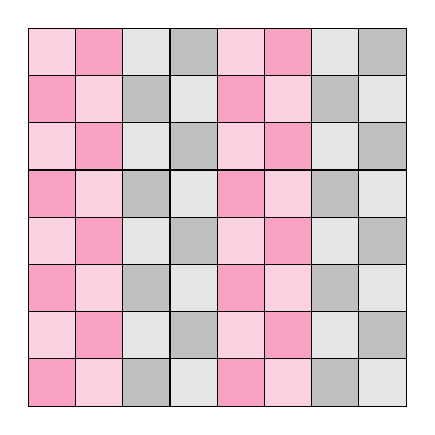
\begin{tikzpicture}[scale=0.6]
			\draw[fill=WildStrawberry, fill opacity=0.4] (0, 0) -- (0, 1) -- (1, 1) -- (1, 0) -- (0, 0);
\draw[fill=WildStrawberry, fill opacity=0.2] (0, 1) -- (0, 2) -- (1, 2) -- (1, 1) -- (0, 1);
\draw[fill=WildStrawberry, fill opacity=0.4] (0, 2) -- (0, 3) -- (1, 3) -- (1, 2) -- (0, 2);
\draw[fill=WildStrawberry, fill opacity=0.2] (0, 3) -- (0, 4) -- (1, 4) -- (1, 3) -- (0, 3);
\draw[fill=WildStrawberry, fill opacity=0.4] (0, 4) -- (0, 5) -- (1, 5) -- (1, 4) -- (0, 4);
\draw[fill=WildStrawberry, fill opacity=0.2] (0, 5) -- (0, 6) -- (1, 6) -- (1, 5) -- (0, 5);
\draw[fill=WildStrawberry, fill opacity=0.4] (0, 6) -- (0, 7) -- (1, 7) -- (1, 6) -- (0, 6);
\draw[fill=WildStrawberry, fill opacity=0.2] (0, 7) -- (0, 8) -- (1, 8) -- (1, 7) -- (0, 7);
\draw[fill=WildStrawberry, fill opacity=0.2] (1, 0) -- (1, 1) -- (2, 1) -- (2, 0) -- (1, 0);
\draw[fill=WildStrawberry, fill opacity=0.4] (1, 1) -- (1, 2) -- (2, 2) -- (2, 1) -- (1, 1);
\draw[fill=WildStrawberry, fill opacity=0.2] (1, 2) -- (1, 3) -- (2, 3) -- (2, 2) -- (1, 2);
\draw[fill=WildStrawberry, fill opacity=0.4] (1, 3) -- (1, 4) -- (2, 4) -- (2, 3) -- (1, 3);
\draw[fill=WildStrawberry, fill opacity=0.2] (1, 4) -- (1, 5) -- (2, 5) -- (2, 4) -- (1, 4);
\draw[fill=WildStrawberry, fill opacity=0.4] (1, 5) -- (1, 6) -- (2, 6) -- (2, 5) -- (1, 5);
\draw[fill=WildStrawberry, fill opacity=0.2] (1, 6) -- (1, 7) -- (2, 7) -- (2, 6) -- (1, 6);
\draw[fill=WildStrawberry, fill opacity=0.4] (1, 7) -- (1, 8) -- (2, 8) -- (2, 7) -- (1, 7);
\draw[fill=black, fill opacity=0.25] (2, 0) -- (2, 1) -- (3, 1) -- (3, 0) -- (2, 0);
\draw[fill=black, fill opacity=0.1] (2, 1) -- (2, 2) -- (3, 2) -- (3, 1) -- (2, 1);
\draw[fill=black, fill opacity=0.25] (2, 2) -- (2, 3) -- (3, 3) -- (3, 2) -- (2, 2);
\draw[fill=black, fill opacity=0.1] (2, 3) -- (2, 4) -- (3, 4) -- (3, 3) -- (2, 3);
\draw[fill=black, fill opacity=0.25] (2, 4) -- (2, 5) -- (3, 5) -- (3, 4) -- (2, 4);
\draw[fill=black, fill opacity=0.1] (2, 5) -- (2, 6) -- (3, 6) -- (3, 5) -- (2, 5);
\draw[fill=black, fill opacity=0.25] (2, 6) -- (2, 7) -- (3, 7) -- (3, 6) -- (2, 6);
\draw[fill=black, fill opacity=0.1] (2, 7) -- (2, 8) -- (3, 8) -- (3, 7) -- (2, 7);
\draw[fill=black, fill opacity=0.1] (3, 0) -- (3, 1) -- (4, 1) -- (4, 0) -- (3, 0);
\draw[fill=black, fill opacity=0.25] (3, 1) -- (3, 2) -- (4, 2) -- (4, 1) -- (3, 1);
\draw[fill=black, fill opacity=0.1] (3, 2) -- (3, 3) -- (4, 3) -- (4, 2) -- (3, 2);
\draw[fill=black, fill opacity=0.25] (3, 3) -- (3, 4) -- (4, 4) -- (4, 3) -- (3, 3);
\draw[fill=black, fill opacity=0.1] (3, 4) -- (3, 5) -- (4, 5) -- (4, 4) -- (3, 4);
\draw[fill=black, fill opacity=0.25] (3, 5) -- (3, 6) -- (4, 6) -- (4, 5) -- (3, 5);
\draw[fill=black, fill opacity=0.1] (3, 6) -- (3, 7) -- (4, 7) -- (4, 6) -- (3, 6);
\draw[fill=black, fill opacity=0.25] (3, 7) -- (3, 8) -- (4, 8) -- (4, 7) -- (3, 7);
\draw[fill=WildStrawberry, fill opacity=0.4] (4, 0) -- (4, 1) -- (5, 1) -- (5, 0) -- (4, 0);
\draw[fill=WildStrawberry, fill opacity=0.2] (4, 1) -- (4, 2) -- (5, 2) -- (5, 1) -- (4, 1);
\draw[fill=WildStrawberry, fill opacity=0.4] (4, 2) -- (4, 3) -- (5, 3) -- (5, 2) -- (4, 2);
\draw[fill=WildStrawberry, fill opacity=0.2] (4, 3) -- (4, 4) -- (5, 4) -- (5, 3) -- (4, 3);
\draw[fill=WildStrawberry, fill opacity=0.4] (4, 4) -- (4, 5) -- (5, 5) -- (5, 4) -- (4, 4);
\draw[fill=WildStrawberry, fill opacity=0.2] (4, 5) -- (4, 6) -- (5, 6) -- (5, 5) -- (4, 5);
\draw[fill=WildStrawberry, fill opacity=0.4] (4, 6) -- (4, 7) -- (5, 7) -- (5, 6) -- (4, 6);
\draw[fill=WildStrawberry, fill opacity=0.2] (4, 7) -- (4, 8) -- (5, 8) -- (5, 7) -- (4, 7);
\draw[fill=WildStrawberry, fill opacity=0.2] (5, 0) -- (5, 1) -- (6, 1) -- (6, 0) -- (5, 0);
\draw[fill=WildStrawberry, fill opacity=0.4] (5, 1) -- (5, 2) -- (6, 2) -- (6, 1) -- (5, 1);
\draw[fill=WildStrawberry, fill opacity=0.2] (5, 2) -- (5, 3) -- (6, 3) -- (6, 2) -- (5, 2);
\draw[fill=WildStrawberry, fill opacity=0.4] (5, 3) -- (5, 4) -- (6, 4) -- (6, 3) -- (5, 3);
\draw[fill=WildStrawberry, fill opacity=0.2] (5, 4) -- (5, 5) -- (6, 5) -- (6, 4) -- (5, 4);
\draw[fill=WildStrawberry, fill opacity=0.4] (5, 5) -- (5, 6) -- (6, 6) -- (6, 5) -- (5, 5);
\draw[fill=WildStrawberry, fill opacity=0.2] (5, 6) -- (5, 7) -- (6, 7) -- (6, 6) -- (5, 6);
\draw[fill=WildStrawberry, fill opacity=0.4] (5, 7) -- (5, 8) -- (6, 8) -- (6, 7) -- (5, 7);
\draw[fill=black, fill opacity=0.25] (6, 0) -- (6, 1) -- (7, 1) -- (7, 0) -- (6, 0);
\draw[fill=black, fill opacity=0.1] (6, 1) -- (6, 2) -- (7, 2) -- (7, 1) -- (6, 1);
\draw[fill=black, fill opacity=0.25] (6, 2) -- (6, 3) -- (7, 3) -- (7, 2) -- (6, 2);
\draw[fill=black, fill opacity=0.1] (6, 3) -- (6, 4) -- (7, 4) -- (7, 3) -- (6, 3);
\draw[fill=black, fill opacity=0.25] (6, 4) -- (6, 5) -- (7, 5) -- (7, 4) -- (6, 4);
\draw[fill=black, fill opacity=0.1] (6, 5) -- (6, 6) -- (7, 6) -- (7, 5) -- (6, 5);
\draw[fill=black, fill opacity=0.25] (6, 6) -- (6, 7) -- (7, 7) -- (7, 6) -- (6, 6);
\draw[fill=black, fill opacity=0.1] (6, 7) -- (6, 8) -- (7, 8) -- (7, 7) -- (6, 7);
\draw[fill=black, fill opacity=0.1] (7, 0) -- (7, 1) -- (8, 1) -- (8, 0) -- (7, 0);
\draw[fill=black, fill opacity=0.25] (7, 1) -- (7, 2) -- (8, 2) -- (8, 1) -- (7, 1);
\draw[fill=black, fill opacity=0.1] (7, 2) -- (7, 3) -- (8, 3) -- (8, 2) -- (7, 2);
\draw[fill=black, fill opacity=0.25] (7, 3) -- (7, 4) -- (8, 4) -- (8, 3) -- (7, 3);
\draw[fill=black, fill opacity=0.1] (7, 4) -- (7, 5) -- (8, 5) -- (8, 4) -- (7, 4);
\draw[fill=black, fill opacity=0.25] (7, 5) -- (7, 6) -- (8, 6) -- (8, 5) -- (7, 5);
\draw[fill=black, fill opacity=0.1] (7, 6) -- (7, 7) -- (8, 7) -- (8, 6) -- (7, 6);
\draw[fill=black, fill opacity=0.25] (7, 7) -- (7, 8) -- (8, 8) -- (8, 7) -- (7, 7);
		\end{tikzpicture}\hspace{5mm}
		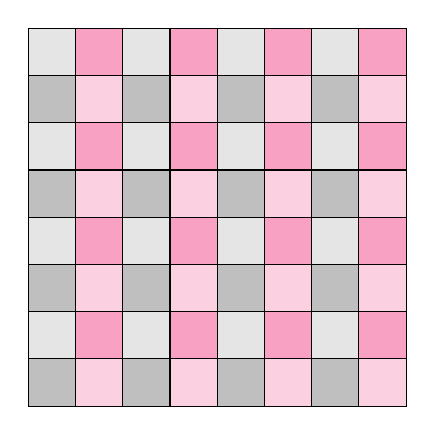
\begin{tikzpicture}[scale=0.6]
			\draw[fill=black, fill opacity=0.25] (0, 0) -- (0, 1) -- (1, 1) -- (1, 0) -- (0, 0);
\draw[fill=WildStrawberry, fill opacity=0.2] (1, 0) -- (1, 1) -- (2, 1) -- (2, 0) -- (1, 0);
\draw[fill=black, fill opacity=0.25] (2, 0) -- (2, 1) -- (3, 1) -- (3, 0) -- (2, 0);
\draw[fill=WildStrawberry, fill opacity=0.2] (3, 0) -- (3, 1) -- (4, 1) -- (4, 0) -- (3, 0);
\draw[fill=black, fill opacity=0.25] (4, 0) -- (4, 1) -- (5, 1) -- (5, 0) -- (4, 0);
\draw[fill=WildStrawberry, fill opacity=0.2] (5, 0) -- (5, 1) -- (6, 1) -- (6, 0) -- (5, 0);
\draw[fill=black, fill opacity=0.25] (6, 0) -- (6, 1) -- (7, 1) -- (7, 0) -- (6, 0);
\draw[fill=WildStrawberry, fill opacity=0.2] (7, 0) -- (7, 1) -- (8, 1) -- (8, 0) -- (7, 0);
\draw[fill=black, fill opacity=0.1] (0, 1) -- (0, 2) -- (1, 2) -- (1, 1) -- (0, 1);
\draw[fill=WildStrawberry, fill opacity=0.4] (1, 1) -- (1, 2) -- (2, 2) -- (2, 1) -- (1, 1);
\draw[fill=black, fill opacity=0.1] (2, 1) -- (2, 2) -- (3, 2) -- (3, 1) -- (2, 1);
\draw[fill=WildStrawberry, fill opacity=0.4] (3, 1) -- (3, 2) -- (4, 2) -- (4, 1) -- (3, 1);
\draw[fill=black, fill opacity=0.1] (4, 1) -- (4, 2) -- (5, 2) -- (5, 1) -- (4, 1);
\draw[fill=WildStrawberry, fill opacity=0.4] (5, 1) -- (5, 2) -- (6, 2) -- (6, 1) -- (5, 1);
\draw[fill=black, fill opacity=0.1] (6, 1) -- (6, 2) -- (7, 2) -- (7, 1) -- (6, 1);
\draw[fill=WildStrawberry, fill opacity=0.4] (7, 1) -- (7, 2) -- (8, 2) -- (8, 1) -- (7, 1);
\draw[fill=black, fill opacity=0.25] (0, 2) -- (0, 3) -- (1, 3) -- (1, 2) -- (0, 2);
\draw[fill=WildStrawberry, fill opacity=0.2] (1, 2) -- (1, 3) -- (2, 3) -- (2, 2) -- (1, 2);
\draw[fill=black, fill opacity=0.25] (2, 2) -- (2, 3) -- (3, 3) -- (3, 2) -- (2, 2);
\draw[fill=WildStrawberry, fill opacity=0.2] (3, 2) -- (3, 3) -- (4, 3) -- (4, 2) -- (3, 2);
\draw[fill=black, fill opacity=0.25] (4, 2) -- (4, 3) -- (5, 3) -- (5, 2) -- (4, 2);
\draw[fill=WildStrawberry, fill opacity=0.2] (5, 2) -- (5, 3) -- (6, 3) -- (6, 2) -- (5, 2);
\draw[fill=black, fill opacity=0.25] (6, 2) -- (6, 3) -- (7, 3) -- (7, 2) -- (6, 2);
\draw[fill=WildStrawberry, fill opacity=0.2] (7, 2) -- (7, 3) -- (8, 3) -- (8, 2) -- (7, 2);
\draw[fill=black, fill opacity=0.1] (0, 3) -- (0, 4) -- (1, 4) -- (1, 3) -- (0, 3);
\draw[fill=WildStrawberry, fill opacity=0.4] (1, 3) -- (1, 4) -- (2, 4) -- (2, 3) -- (1, 3);
\draw[fill=black, fill opacity=0.1] (2, 3) -- (2, 4) -- (3, 4) -- (3, 3) -- (2, 3);
\draw[fill=WildStrawberry, fill opacity=0.4] (3, 3) -- (3, 4) -- (4, 4) -- (4, 3) -- (3, 3);
\draw[fill=black, fill opacity=0.1] (4, 3) -- (4, 4) -- (5, 4) -- (5, 3) -- (4, 3);
\draw[fill=WildStrawberry, fill opacity=0.4] (5, 3) -- (5, 4) -- (6, 4) -- (6, 3) -- (5, 3);
\draw[fill=black, fill opacity=0.1] (6, 3) -- (6, 4) -- (7, 4) -- (7, 3) -- (6, 3);
\draw[fill=WildStrawberry, fill opacity=0.4] (7, 3) -- (7, 4) -- (8, 4) -- (8, 3) -- (7, 3);
\draw[fill=black, fill opacity=0.25] (0, 4) -- (0, 5) -- (1, 5) -- (1, 4) -- (0, 4);
\draw[fill=WildStrawberry, fill opacity=0.2] (1, 4) -- (1, 5) -- (2, 5) -- (2, 4) -- (1, 4);
\draw[fill=black, fill opacity=0.25] (2, 4) -- (2, 5) -- (3, 5) -- (3, 4) -- (2, 4);
\draw[fill=WildStrawberry, fill opacity=0.2] (3, 4) -- (3, 5) -- (4, 5) -- (4, 4) -- (3, 4);
\draw[fill=black, fill opacity=0.25] (4, 4) -- (4, 5) -- (5, 5) -- (5, 4) -- (4, 4);
\draw[fill=WildStrawberry, fill opacity=0.2] (5, 4) -- (5, 5) -- (6, 5) -- (6, 4) -- (5, 4);
\draw[fill=black, fill opacity=0.25] (6, 4) -- (6, 5) -- (7, 5) -- (7, 4) -- (6, 4);
\draw[fill=WildStrawberry, fill opacity=0.2] (7, 4) -- (7, 5) -- (8, 5) -- (8, 4) -- (7, 4);
\draw[fill=black, fill opacity=0.1] (0, 5) -- (0, 6) -- (1, 6) -- (1, 5) -- (0, 5);
\draw[fill=WildStrawberry, fill opacity=0.4] (1, 5) -- (1, 6) -- (2, 6) -- (2, 5) -- (1, 5);
\draw[fill=black, fill opacity=0.1] (2, 5) -- (2, 6) -- (3, 6) -- (3, 5) -- (2, 5);
\draw[fill=WildStrawberry, fill opacity=0.4] (3, 5) -- (3, 6) -- (4, 6) -- (4, 5) -- (3, 5);
\draw[fill=black, fill opacity=0.1] (4, 5) -- (4, 6) -- (5, 6) -- (5, 5) -- (4, 5);
\draw[fill=WildStrawberry, fill opacity=0.4] (5, 5) -- (5, 6) -- (6, 6) -- (6, 5) -- (5, 5);
\draw[fill=black, fill opacity=0.1] (6, 5) -- (6, 6) -- (7, 6) -- (7, 5) -- (6, 5);
\draw[fill=WildStrawberry, fill opacity=0.4] (7, 5) -- (7, 6) -- (8, 6) -- (8, 5) -- (7, 5);
\draw[fill=black, fill opacity=0.25] (0, 6) -- (0, 7) -- (1, 7) -- (1, 6) -- (0, 6);
\draw[fill=WildStrawberry, fill opacity=0.2] (1, 6) -- (1, 7) -- (2, 7) -- (2, 6) -- (1, 6);
\draw[fill=black, fill opacity=0.25] (2, 6) -- (2, 7) -- (3, 7) -- (3, 6) -- (2, 6);
\draw[fill=WildStrawberry, fill opacity=0.2] (3, 6) -- (3, 7) -- (4, 7) -- (4, 6) -- (3, 6);
\draw[fill=black, fill opacity=0.25] (4, 6) -- (4, 7) -- (5, 7) -- (5, 6) -- (4, 6);
\draw[fill=WildStrawberry, fill opacity=0.2] (5, 6) -- (5, 7) -- (6, 7) -- (6, 6) -- (5, 6);
\draw[fill=black, fill opacity=0.25] (6, 6) -- (6, 7) -- (7, 7) -- (7, 6) -- (6, 6);
\draw[fill=WildStrawberry, fill opacity=0.2] (7, 6) -- (7, 7) -- (8, 7) -- (8, 6) -- (7, 6);
\draw[fill=black, fill opacity=0.1] (0, 7) -- (0, 8) -- (1, 8) -- (1, 7) -- (0, 7);
\draw[fill=WildStrawberry, fill opacity=0.4] (1, 7) -- (1, 8) -- (2, 8) -- (2, 7) -- (1, 7);
\draw[fill=black, fill opacity=0.1] (2, 7) -- (2, 8) -- (3, 8) -- (3, 7) -- (2, 7);
\draw[fill=WildStrawberry, fill opacity=0.4] (3, 7) -- (3, 8) -- (4, 8) -- (4, 7) -- (3, 7);
\draw[fill=black, fill opacity=0.1] (4, 7) -- (4, 8) -- (5, 8) -- (5, 7) -- (4, 7);
\draw[fill=WildStrawberry, fill opacity=0.4] (5, 7) -- (5, 8) -- (6, 8) -- (6, 7) -- (5, 7);
\draw[fill=black, fill opacity=0.1] (6, 7) -- (6, 8) -- (7, 8) -- (7, 7) -- (6, 7);
\draw[fill=WildStrawberry, fill opacity=0.4] (7, 7) -- (7, 8) -- (8, 8) -- (8, 7) -- (7, 7);
		\end{tikzpicture}
		\vspace{5mm}\\
		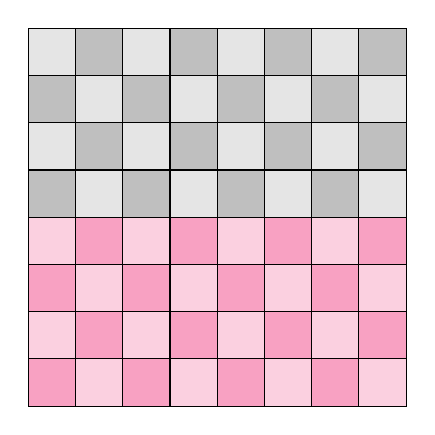
\begin{tikzpicture}[scale=0.6]
			\draw[fill=WildStrawberry, fill opacity=0.4] (0, 0) -- (0, 1) -- (1, 1) -- (1, 0) -- (0, 0);
\draw[fill=WildStrawberry, fill opacity=0.2] (1, 0) -- (1, 1) -- (2, 1) -- (2, 0) -- (1, 0);
\draw[fill=WildStrawberry, fill opacity=0.4] (2, 0) -- (2, 1) -- (3, 1) -- (3, 0) -- (2, 0);
\draw[fill=WildStrawberry, fill opacity=0.2] (3, 0) -- (3, 1) -- (4, 1) -- (4, 0) -- (3, 0);
\draw[fill=WildStrawberry, fill opacity=0.4] (4, 0) -- (4, 1) -- (5, 1) -- (5, 0) -- (4, 0);
\draw[fill=WildStrawberry, fill opacity=0.2] (5, 0) -- (5, 1) -- (6, 1) -- (6, 0) -- (5, 0);
\draw[fill=WildStrawberry, fill opacity=0.4] (6, 0) -- (6, 1) -- (7, 1) -- (7, 0) -- (6, 0);
\draw[fill=WildStrawberry, fill opacity=0.2] (7, 0) -- (7, 1) -- (8, 1) -- (8, 0) -- (7, 0);
\draw[fill=WildStrawberry, fill opacity=0.2] (0, 1) -- (0, 2) -- (1, 2) -- (1, 1) -- (0, 1);
\draw[fill=WildStrawberry, fill opacity=0.4] (1, 1) -- (1, 2) -- (2, 2) -- (2, 1) -- (1, 1);
\draw[fill=WildStrawberry, fill opacity=0.2] (2, 1) -- (2, 2) -- (3, 2) -- (3, 1) -- (2, 1);
\draw[fill=WildStrawberry, fill opacity=0.4] (3, 1) -- (3, 2) -- (4, 2) -- (4, 1) -- (3, 1);
\draw[fill=WildStrawberry, fill opacity=0.2] (4, 1) -- (4, 2) -- (5, 2) -- (5, 1) -- (4, 1);
\draw[fill=WildStrawberry, fill opacity=0.4] (5, 1) -- (5, 2) -- (6, 2) -- (6, 1) -- (5, 1);
\draw[fill=WildStrawberry, fill opacity=0.2] (6, 1) -- (6, 2) -- (7, 2) -- (7, 1) -- (6, 1);
\draw[fill=WildStrawberry, fill opacity=0.4] (7, 1) -- (7, 2) -- (8, 2) -- (8, 1) -- (7, 1);
\draw[fill=WildStrawberry, fill opacity=0.4] (0, 2) -- (0, 3) -- (1, 3) -- (1, 2) -- (0, 2);
\draw[fill=WildStrawberry, fill opacity=0.2] (1, 2) -- (1, 3) -- (2, 3) -- (2, 2) -- (1, 2);
\draw[fill=WildStrawberry, fill opacity=0.4] (2, 2) -- (2, 3) -- (3, 3) -- (3, 2) -- (2, 2);
\draw[fill=WildStrawberry, fill opacity=0.2] (3, 2) -- (3, 3) -- (4, 3) -- (4, 2) -- (3, 2);
\draw[fill=WildStrawberry, fill opacity=0.4] (4, 2) -- (4, 3) -- (5, 3) -- (5, 2) -- (4, 2);
\draw[fill=WildStrawberry, fill opacity=0.2] (5, 2) -- (5, 3) -- (6, 3) -- (6, 2) -- (5, 2);
\draw[fill=WildStrawberry, fill opacity=0.4] (6, 2) -- (6, 3) -- (7, 3) -- (7, 2) -- (6, 2);
\draw[fill=WildStrawberry, fill opacity=0.2] (7, 2) -- (7, 3) -- (8, 3) -- (8, 2) -- (7, 2);
\draw[fill=WildStrawberry, fill opacity=0.2] (0, 3) -- (0, 4) -- (1, 4) -- (1, 3) -- (0, 3);
\draw[fill=WildStrawberry, fill opacity=0.4] (1, 3) -- (1, 4) -- (2, 4) -- (2, 3) -- (1, 3);
\draw[fill=WildStrawberry, fill opacity=0.2] (2, 3) -- (2, 4) -- (3, 4) -- (3, 3) -- (2, 3);
\draw[fill=WildStrawberry, fill opacity=0.4] (3, 3) -- (3, 4) -- (4, 4) -- (4, 3) -- (3, 3);
\draw[fill=WildStrawberry, fill opacity=0.2] (4, 3) -- (4, 4) -- (5, 4) -- (5, 3) -- (4, 3);
\draw[fill=WildStrawberry, fill opacity=0.4] (5, 3) -- (5, 4) -- (6, 4) -- (6, 3) -- (5, 3);
\draw[fill=WildStrawberry, fill opacity=0.2] (6, 3) -- (6, 4) -- (7, 4) -- (7, 3) -- (6, 3);
\draw[fill=WildStrawberry, fill opacity=0.4] (7, 3) -- (7, 4) -- (8, 4) -- (8, 3) -- (7, 3);
\draw[fill=black, fill opacity=0.25] (0, 4) -- (0, 5) -- (1, 5) -- (1, 4) -- (0, 4);
\draw[fill=black, fill opacity=0.1] (1, 4) -- (1, 5) -- (2, 5) -- (2, 4) -- (1, 4);
\draw[fill=black, fill opacity=0.25] (2, 4) -- (2, 5) -- (3, 5) -- (3, 4) -- (2, 4);
\draw[fill=black, fill opacity=0.1] (3, 4) -- (3, 5) -- (4, 5) -- (4, 4) -- (3, 4);
\draw[fill=black, fill opacity=0.25] (4, 4) -- (4, 5) -- (5, 5) -- (5, 4) -- (4, 4);
\draw[fill=black, fill opacity=0.1] (5, 4) -- (5, 5) -- (6, 5) -- (6, 4) -- (5, 4);
\draw[fill=black, fill opacity=0.25] (6, 4) -- (6, 5) -- (7, 5) -- (7, 4) -- (6, 4);
\draw[fill=black, fill opacity=0.1] (7, 4) -- (7, 5) -- (8, 5) -- (8, 4) -- (7, 4);
\draw[fill=black, fill opacity=0.1] (0, 5) -- (0, 6) -- (1, 6) -- (1, 5) -- (0, 5);
\draw[fill=black, fill opacity=0.25] (1, 5) -- (1, 6) -- (2, 6) -- (2, 5) -- (1, 5);
\draw[fill=black, fill opacity=0.1] (2, 5) -- (2, 6) -- (3, 6) -- (3, 5) -- (2, 5);
\draw[fill=black, fill opacity=0.25] (3, 5) -- (3, 6) -- (4, 6) -- (4, 5) -- (3, 5);
\draw[fill=black, fill opacity=0.1] (4, 5) -- (4, 6) -- (5, 6) -- (5, 5) -- (4, 5);
\draw[fill=black, fill opacity=0.25] (5, 5) -- (5, 6) -- (6, 6) -- (6, 5) -- (5, 5);
\draw[fill=black, fill opacity=0.1] (6, 5) -- (6, 6) -- (7, 6) -- (7, 5) -- (6, 5);
\draw[fill=black, fill opacity=0.25] (7, 5) -- (7, 6) -- (8, 6) -- (8, 5) -- (7, 5);
\draw[fill=black, fill opacity=0.25] (0, 6) -- (0, 7) -- (1, 7) -- (1, 6) -- (0, 6);
\draw[fill=black, fill opacity=0.1] (1, 6) -- (1, 7) -- (2, 7) -- (2, 6) -- (1, 6);
\draw[fill=black, fill opacity=0.25] (2, 6) -- (2, 7) -- (3, 7) -- (3, 6) -- (2, 6);
\draw[fill=black, fill opacity=0.1] (3, 6) -- (3, 7) -- (4, 7) -- (4, 6) -- (3, 6);
\draw[fill=black, fill opacity=0.25] (4, 6) -- (4, 7) -- (5, 7) -- (5, 6) -- (4, 6);
\draw[fill=black, fill opacity=0.1] (5, 6) -- (5, 7) -- (6, 7) -- (6, 6) -- (5, 6);
\draw[fill=black, fill opacity=0.25] (6, 6) -- (6, 7) -- (7, 7) -- (7, 6) -- (6, 6);
\draw[fill=black, fill opacity=0.1] (7, 6) -- (7, 7) -- (8, 7) -- (8, 6) -- (7, 6);
\draw[fill=black, fill opacity=0.1] (0, 7) -- (0, 8) -- (1, 8) -- (1, 7) -- (0, 7);
\draw[fill=black, fill opacity=0.25] (1, 7) -- (1, 8) -- (2, 8) -- (2, 7) -- (1, 7);
\draw[fill=black, fill opacity=0.1] (2, 7) -- (2, 8) -- (3, 8) -- (3, 7) -- (2, 7);
\draw[fill=black, fill opacity=0.25] (3, 7) -- (3, 8) -- (4, 8) -- (4, 7) -- (3, 7);
\draw[fill=black, fill opacity=0.1] (4, 7) -- (4, 8) -- (5, 8) -- (5, 7) -- (4, 7);
\draw[fill=black, fill opacity=0.25] (5, 7) -- (5, 8) -- (6, 8) -- (6, 7) -- (5, 7);
\draw[fill=black, fill opacity=0.1] (6, 7) -- (6, 8) -- (7, 8) -- (7, 7) -- (6, 7);
\draw[fill=black, fill opacity=0.25] (7, 7) -- (7, 8) -- (8, 8) -- (8, 7) -- (7, 7);
		\end{tikzpicture}\hspace{5mm}
		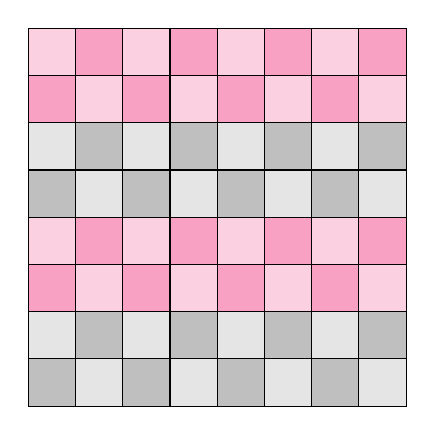
\begin{tikzpicture}[scale=0.6]
			\draw[fill=black, fill opacity=0.25] (0, 0) -- (0, 1) -- (1, 1) -- (1, 0) -- (0, 0);
\draw[fill=black, fill opacity=0.1] (0, 1) -- (0, 2) -- (1, 2) -- (1, 1) -- (0, 1);
\draw[fill=WildStrawberry, fill opacity=0.4] (0, 2) -- (0, 3) -- (1, 3) -- (1, 2) -- (0, 2);
\draw[fill=WildStrawberry, fill opacity=0.2] (0, 3) -- (0, 4) -- (1, 4) -- (1, 3) -- (0, 3);
\draw[fill=black, fill opacity=0.25] (0, 4) -- (0, 5) -- (1, 5) -- (1, 4) -- (0, 4);
\draw[fill=black, fill opacity=0.1] (0, 5) -- (0, 6) -- (1, 6) -- (1, 5) -- (0, 5);
\draw[fill=WildStrawberry, fill opacity=0.4] (0, 6) -- (0, 7) -- (1, 7) -- (1, 6) -- (0, 6);
\draw[fill=WildStrawberry, fill opacity=0.2] (0, 7) -- (0, 8) -- (1, 8) -- (1, 7) -- (0, 7);
\draw[fill=black, fill opacity=0.1] (1, 0) -- (1, 1) -- (2, 1) -- (2, 0) -- (1, 0);
\draw[fill=black, fill opacity=0.25] (1, 1) -- (1, 2) -- (2, 2) -- (2, 1) -- (1, 1);
\draw[fill=WildStrawberry, fill opacity=0.2] (1, 2) -- (1, 3) -- (2, 3) -- (2, 2) -- (1, 2);
\draw[fill=WildStrawberry, fill opacity=0.4] (1, 3) -- (1, 4) -- (2, 4) -- (2, 3) -- (1, 3);
\draw[fill=black, fill opacity=0.1] (1, 4) -- (1, 5) -- (2, 5) -- (2, 4) -- (1, 4);
\draw[fill=black, fill opacity=0.25] (1, 5) -- (1, 6) -- (2, 6) -- (2, 5) -- (1, 5);
\draw[fill=WildStrawberry, fill opacity=0.2] (1, 6) -- (1, 7) -- (2, 7) -- (2, 6) -- (1, 6);
\draw[fill=WildStrawberry, fill opacity=0.4] (1, 7) -- (1, 8) -- (2, 8) -- (2, 7) -- (1, 7);
\draw[fill=black, fill opacity=0.25] (2, 0) -- (2, 1) -- (3, 1) -- (3, 0) -- (2, 0);
\draw[fill=black, fill opacity=0.1] (2, 1) -- (2, 2) -- (3, 2) -- (3, 1) -- (2, 1);
\draw[fill=WildStrawberry, fill opacity=0.4] (2, 2) -- (2, 3) -- (3, 3) -- (3, 2) -- (2, 2);
\draw[fill=WildStrawberry, fill opacity=0.2] (2, 3) -- (2, 4) -- (3, 4) -- (3, 3) -- (2, 3);
\draw[fill=black, fill opacity=0.25] (2, 4) -- (2, 5) -- (3, 5) -- (3, 4) -- (2, 4);
\draw[fill=black, fill opacity=0.1] (2, 5) -- (2, 6) -- (3, 6) -- (3, 5) -- (2, 5);
\draw[fill=WildStrawberry, fill opacity=0.4] (2, 6) -- (2, 7) -- (3, 7) -- (3, 6) -- (2, 6);
\draw[fill=WildStrawberry, fill opacity=0.2] (2, 7) -- (2, 8) -- (3, 8) -- (3, 7) -- (2, 7);
\draw[fill=black, fill opacity=0.1] (3, 0) -- (3, 1) -- (4, 1) -- (4, 0) -- (3, 0);
\draw[fill=black, fill opacity=0.25] (3, 1) -- (3, 2) -- (4, 2) -- (4, 1) -- (3, 1);
\draw[fill=WildStrawberry, fill opacity=0.2] (3, 2) -- (3, 3) -- (4, 3) -- (4, 2) -- (3, 2);
\draw[fill=WildStrawberry, fill opacity=0.4] (3, 3) -- (3, 4) -- (4, 4) -- (4, 3) -- (3, 3);
\draw[fill=black, fill opacity=0.1] (3, 4) -- (3, 5) -- (4, 5) -- (4, 4) -- (3, 4);
\draw[fill=black, fill opacity=0.25] (3, 5) -- (3, 6) -- (4, 6) -- (4, 5) -- (3, 5);
\draw[fill=WildStrawberry, fill opacity=0.2] (3, 6) -- (3, 7) -- (4, 7) -- (4, 6) -- (3, 6);
\draw[fill=WildStrawberry, fill opacity=0.4] (3, 7) -- (3, 8) -- (4, 8) -- (4, 7) -- (3, 7);
\draw[fill=black, fill opacity=0.25] (4, 0) -- (4, 1) -- (5, 1) -- (5, 0) -- (4, 0);
\draw[fill=black, fill opacity=0.1] (4, 1) -- (4, 2) -- (5, 2) -- (5, 1) -- (4, 1);
\draw[fill=WildStrawberry, fill opacity=0.4] (4, 2) -- (4, 3) -- (5, 3) -- (5, 2) -- (4, 2);
\draw[fill=WildStrawberry, fill opacity=0.2] (4, 3) -- (4, 4) -- (5, 4) -- (5, 3) -- (4, 3);
\draw[fill=black, fill opacity=0.25] (4, 4) -- (4, 5) -- (5, 5) -- (5, 4) -- (4, 4);
\draw[fill=black, fill opacity=0.1] (4, 5) -- (4, 6) -- (5, 6) -- (5, 5) -- (4, 5);
\draw[fill=WildStrawberry, fill opacity=0.4] (4, 6) -- (4, 7) -- (5, 7) -- (5, 6) -- (4, 6);
\draw[fill=WildStrawberry, fill opacity=0.2] (4, 7) -- (4, 8) -- (5, 8) -- (5, 7) -- (4, 7);
\draw[fill=black, fill opacity=0.1] (5, 0) -- (5, 1) -- (6, 1) -- (6, 0) -- (5, 0);
\draw[fill=black, fill opacity=0.25] (5, 1) -- (5, 2) -- (6, 2) -- (6, 1) -- (5, 1);
\draw[fill=WildStrawberry, fill opacity=0.2] (5, 2) -- (5, 3) -- (6, 3) -- (6, 2) -- (5, 2);
\draw[fill=WildStrawberry, fill opacity=0.4] (5, 3) -- (5, 4) -- (6, 4) -- (6, 3) -- (5, 3);
\draw[fill=black, fill opacity=0.1] (5, 4) -- (5, 5) -- (6, 5) -- (6, 4) -- (5, 4);
\draw[fill=black, fill opacity=0.25] (5, 5) -- (5, 6) -- (6, 6) -- (6, 5) -- (5, 5);
\draw[fill=WildStrawberry, fill opacity=0.2] (5, 6) -- (5, 7) -- (6, 7) -- (6, 6) -- (5, 6);
\draw[fill=WildStrawberry, fill opacity=0.4] (5, 7) -- (5, 8) -- (6, 8) -- (6, 7) -- (5, 7);
\draw[fill=black, fill opacity=0.25] (6, 0) -- (6, 1) -- (7, 1) -- (7, 0) -- (6, 0);
\draw[fill=black, fill opacity=0.1] (6, 1) -- (6, 2) -- (7, 2) -- (7, 1) -- (6, 1);
\draw[fill=WildStrawberry, fill opacity=0.4] (6, 2) -- (6, 3) -- (7, 3) -- (7, 2) -- (6, 2);
\draw[fill=WildStrawberry, fill opacity=0.2] (6, 3) -- (6, 4) -- (7, 4) -- (7, 3) -- (6, 3);
\draw[fill=black, fill opacity=0.25] (6, 4) -- (6, 5) -- (7, 5) -- (7, 4) -- (6, 4);
\draw[fill=black, fill opacity=0.1] (6, 5) -- (6, 6) -- (7, 6) -- (7, 5) -- (6, 5);
\draw[fill=WildStrawberry, fill opacity=0.4] (6, 6) -- (6, 7) -- (7, 7) -- (7, 6) -- (6, 6);
\draw[fill=WildStrawberry, fill opacity=0.2] (6, 7) -- (6, 8) -- (7, 8) -- (7, 7) -- (6, 7);
\draw[fill=black, fill opacity=0.1] (7, 0) -- (7, 1) -- (8, 1) -- (8, 0) -- (7, 0);
\draw[fill=black, fill opacity=0.25] (7, 1) -- (7, 2) -- (8, 2) -- (8, 1) -- (7, 1);
\draw[fill=WildStrawberry, fill opacity=0.2] (7, 2) -- (7, 3) -- (8, 3) -- (8, 2) -- (7, 2);
\draw[fill=WildStrawberry, fill opacity=0.4] (7, 3) -- (7, 4) -- (8, 4) -- (8, 3) -- (7, 3);
\draw[fill=black, fill opacity=0.1] (7, 4) -- (7, 5) -- (8, 5) -- (8, 4) -- (7, 4);
\draw[fill=black, fill opacity=0.25] (7, 5) -- (7, 6) -- (8, 6) -- (8, 5) -- (7, 5);
\draw[fill=WildStrawberry, fill opacity=0.2] (7, 6) -- (7, 7) -- (8, 7) -- (8, 6) -- (7, 6);
\draw[fill=WildStrawberry, fill opacity=0.4] (7, 7) -- (7, 8) -- (8, 8) -- (8, 7) -- (7, 7);
		\end{tikzpicture}\hspace{5mm}
		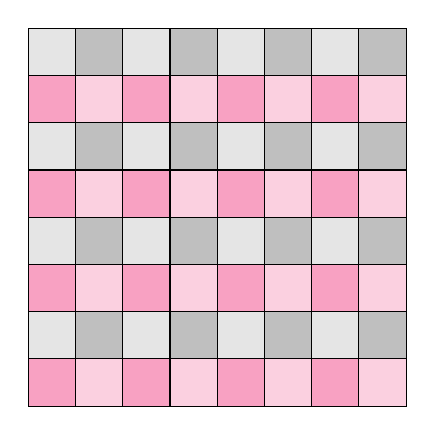
\begin{tikzpicture}[scale=0.6]
			\draw[fill=WildStrawberry, fill opacity=0.4] (0, 0) -- (0, 1) -- (1, 1) -- (1, 0) -- (0, 0);
\draw[fill=WildStrawberry, fill opacity=0.2] (1, 0) -- (1, 1) -- (2, 1) -- (2, 0) -- (1, 0);
\draw[fill=WildStrawberry, fill opacity=0.4] (2, 0) -- (2, 1) -- (3, 1) -- (3, 0) -- (2, 0);
\draw[fill=WildStrawberry, fill opacity=0.2] (3, 0) -- (3, 1) -- (4, 1) -- (4, 0) -- (3, 0);
\draw[fill=WildStrawberry, fill opacity=0.4] (4, 0) -- (4, 1) -- (5, 1) -- (5, 0) -- (4, 0);
\draw[fill=WildStrawberry, fill opacity=0.2] (5, 0) -- (5, 1) -- (6, 1) -- (6, 0) -- (5, 0);
\draw[fill=WildStrawberry, fill opacity=0.4] (6, 0) -- (6, 1) -- (7, 1) -- (7, 0) -- (6, 0);
\draw[fill=WildStrawberry, fill opacity=0.2] (7, 0) -- (7, 1) -- (8, 1) -- (8, 0) -- (7, 0);
\draw[fill=black, fill opacity=0.1] (0, 1) -- (0, 2) -- (1, 2) -- (1, 1) -- (0, 1);
\draw[fill=black, fill opacity=0.25] (1, 1) -- (1, 2) -- (2, 2) -- (2, 1) -- (1, 1);
\draw[fill=black, fill opacity=0.1] (2, 1) -- (2, 2) -- (3, 2) -- (3, 1) -- (2, 1);
\draw[fill=black, fill opacity=0.25] (3, 1) -- (3, 2) -- (4, 2) -- (4, 1) -- (3, 1);
\draw[fill=black, fill opacity=0.1] (4, 1) -- (4, 2) -- (5, 2) -- (5, 1) -- (4, 1);
\draw[fill=black, fill opacity=0.25] (5, 1) -- (5, 2) -- (6, 2) -- (6, 1) -- (5, 1);
\draw[fill=black, fill opacity=0.1] (6, 1) -- (6, 2) -- (7, 2) -- (7, 1) -- (6, 1);
\draw[fill=black, fill opacity=0.25] (7, 1) -- (7, 2) -- (8, 2) -- (8, 1) -- (7, 1);
\draw[fill=WildStrawberry, fill opacity=0.4] (0, 2) -- (0, 3) -- (1, 3) -- (1, 2) -- (0, 2);
\draw[fill=WildStrawberry, fill opacity=0.2] (1, 2) -- (1, 3) -- (2, 3) -- (2, 2) -- (1, 2);
\draw[fill=WildStrawberry, fill opacity=0.4] (2, 2) -- (2, 3) -- (3, 3) -- (3, 2) -- (2, 2);
\draw[fill=WildStrawberry, fill opacity=0.2] (3, 2) -- (3, 3) -- (4, 3) -- (4, 2) -- (3, 2);
\draw[fill=WildStrawberry, fill opacity=0.4] (4, 2) -- (4, 3) -- (5, 3) -- (5, 2) -- (4, 2);
\draw[fill=WildStrawberry, fill opacity=0.2] (5, 2) -- (5, 3) -- (6, 3) -- (6, 2) -- (5, 2);
\draw[fill=WildStrawberry, fill opacity=0.4] (6, 2) -- (6, 3) -- (7, 3) -- (7, 2) -- (6, 2);
\draw[fill=WildStrawberry, fill opacity=0.2] (7, 2) -- (7, 3) -- (8, 3) -- (8, 2) -- (7, 2);
\draw[fill=black, fill opacity=0.1] (0, 3) -- (0, 4) -- (1, 4) -- (1, 3) -- (0, 3);
\draw[fill=black, fill opacity=0.25] (1, 3) -- (1, 4) -- (2, 4) -- (2, 3) -- (1, 3);
\draw[fill=black, fill opacity=0.1] (2, 3) -- (2, 4) -- (3, 4) -- (3, 3) -- (2, 3);
\draw[fill=black, fill opacity=0.25] (3, 3) -- (3, 4) -- (4, 4) -- (4, 3) -- (3, 3);
\draw[fill=black, fill opacity=0.1] (4, 3) -- (4, 4) -- (5, 4) -- (5, 3) -- (4, 3);
\draw[fill=black, fill opacity=0.25] (5, 3) -- (5, 4) -- (6, 4) -- (6, 3) -- (5, 3);
\draw[fill=black, fill opacity=0.1] (6, 3) -- (6, 4) -- (7, 4) -- (7, 3) -- (6, 3);
\draw[fill=black, fill opacity=0.25] (7, 3) -- (7, 4) -- (8, 4) -- (8, 3) -- (7, 3);
\draw[fill=WildStrawberry, fill opacity=0.4] (0, 4) -- (0, 5) -- (1, 5) -- (1, 4) -- (0, 4);
\draw[fill=WildStrawberry, fill opacity=0.2] (1, 4) -- (1, 5) -- (2, 5) -- (2, 4) -- (1, 4);
\draw[fill=WildStrawberry, fill opacity=0.4] (2, 4) -- (2, 5) -- (3, 5) -- (3, 4) -- (2, 4);
\draw[fill=WildStrawberry, fill opacity=0.2] (3, 4) -- (3, 5) -- (4, 5) -- (4, 4) -- (3, 4);
\draw[fill=WildStrawberry, fill opacity=0.4] (4, 4) -- (4, 5) -- (5, 5) -- (5, 4) -- (4, 4);
\draw[fill=WildStrawberry, fill opacity=0.2] (5, 4) -- (5, 5) -- (6, 5) -- (6, 4) -- (5, 4);
\draw[fill=WildStrawberry, fill opacity=0.4] (6, 4) -- (6, 5) -- (7, 5) -- (7, 4) -- (6, 4);
\draw[fill=WildStrawberry, fill opacity=0.2] (7, 4) -- (7, 5) -- (8, 5) -- (8, 4) -- (7, 4);
\draw[fill=black, fill opacity=0.1] (0, 5) -- (0, 6) -- (1, 6) -- (1, 5) -- (0, 5);
\draw[fill=black, fill opacity=0.25] (1, 5) -- (1, 6) -- (2, 6) -- (2, 5) -- (1, 5);
\draw[fill=black, fill opacity=0.1] (2, 5) -- (2, 6) -- (3, 6) -- (3, 5) -- (2, 5);
\draw[fill=black, fill opacity=0.25] (3, 5) -- (3, 6) -- (4, 6) -- (4, 5) -- (3, 5);
\draw[fill=black, fill opacity=0.1] (4, 5) -- (4, 6) -- (5, 6) -- (5, 5) -- (4, 5);
\draw[fill=black, fill opacity=0.25] (5, 5) -- (5, 6) -- (6, 6) -- (6, 5) -- (5, 5);
\draw[fill=black, fill opacity=0.1] (6, 5) -- (6, 6) -- (7, 6) -- (7, 5) -- (6, 5);
\draw[fill=black, fill opacity=0.25] (7, 5) -- (7, 6) -- (8, 6) -- (8, 5) -- (7, 5);
\draw[fill=WildStrawberry, fill opacity=0.4] (0, 6) -- (0, 7) -- (1, 7) -- (1, 6) -- (0, 6);
\draw[fill=WildStrawberry, fill opacity=0.2] (1, 6) -- (1, 7) -- (2, 7) -- (2, 6) -- (1, 6);
\draw[fill=WildStrawberry, fill opacity=0.4] (2, 6) -- (2, 7) -- (3, 7) -- (3, 6) -- (2, 6);
\draw[fill=WildStrawberry, fill opacity=0.2] (3, 6) -- (3, 7) -- (4, 7) -- (4, 6) -- (3, 6);
\draw[fill=WildStrawberry, fill opacity=0.4] (4, 6) -- (4, 7) -- (5, 7) -- (5, 6) -- (4, 6);
\draw[fill=WildStrawberry, fill opacity=0.2] (5, 6) -- (5, 7) -- (6, 7) -- (6, 6) -- (5, 6);
\draw[fill=WildStrawberry, fill opacity=0.4] (6, 6) -- (6, 7) -- (7, 7) -- (7, 6) -- (6, 6);
\draw[fill=WildStrawberry, fill opacity=0.2] (7, 6) -- (7, 7) -- (8, 7) -- (8, 6) -- (7, 6);
\draw[fill=black, fill opacity=0.1] (0, 7) -- (0, 8) -- (1, 8) -- (1, 7) -- (0, 7);
\draw[fill=black, fill opacity=0.25] (1, 7) -- (1, 8) -- (2, 8) -- (2, 7) -- (1, 7);
\draw[fill=black, fill opacity=0.1] (2, 7) -- (2, 8) -- (3, 8) -- (3, 7) -- (2, 7);
\draw[fill=black, fill opacity=0.25] (3, 7) -- (3, 8) -- (4, 8) -- (4, 7) -- (3, 7);
\draw[fill=black, fill opacity=0.1] (4, 7) -- (4, 8) -- (5, 8) -- (5, 7) -- (4, 7);
\draw[fill=black, fill opacity=0.25] (5, 7) -- (5, 8) -- (6, 8) -- (6, 7) -- (5, 7);
\draw[fill=black, fill opacity=0.1] (6, 7) -- (6, 8) -- (7, 8) -- (7, 7) -- (6, 7);
\draw[fill=black, fill opacity=0.25] (7, 7) -- (7, 8) -- (8, 8) -- (8, 7) -- (7, 7);
		\end{tikzpicture}
	\end{center}
\end{figure}

\textbf{Extensions and Comments:}






















